\chapter{The {\tt monsvc} library} % Titlul capotilului
\label{Capitolul2}

The goal of my master project is to implement a library used by the applications to publish monitoring information to the IS servers \citep{kolosinformation}. This section is a brief overview of the functionality of the library. The following sections will present more details about specific aspects of the implementation such as configuration, scheduling and synchronization.

A data taking session of an LHC production fill lasts between 10 and 20 hours. During this time it is important to be able to monitor different operational parameters of the ATLAS TDAQ system and to react to abnormal conditions. For example, one needs to readjust parameters of the event selection software if the acceptance rate becomes so high that persistence services cannot handle it. 

To this end, all the applications in the system need to provide real-time updates about their operational conditions. These updates consist of (multidimensional) histograms, counters, rates, boolean variables, strings and collections thereof - we will refer to them as \emph{monitored objects}. Some examples of such objects are a counter of wrong checksums for event data read from the L1 filter or a histogram of the event sizes for the events accepted by the L2 filter. The updates are sent either periodically, or on demand: at the end of the run, when some exceptional condition occurs or when requested by the operator.

The {\tt monsvc} library takes care of the periodic publication of the monitored information, completely abstracting this task and leaving the application programmer in charge of solely updating the information with the current operational values. This is beneficial since the monitoring information is updated more often and more irregularly than it is published. For example, the counter of wrong checksums is updated every time such an error occurs, but it is expected to be published every 5 seconds. The interval between two publications of a monitored object is called call publishing interval.

In the monsvc approach, the monitoring is split into two operations: registration and publishing. The registration consists of passing a reference to an object to be monitored together with a name for that object to the monsvc library. The publishing deals with sending the data periodically to an IS server from where other applications will read it and either present it to the user or take corrective actions upon failures. 

The programmer needs to register the monitored objects (via the {\tt MonitoringService}), to configure the publishing process and to start it (via the {\tt PublishingController}). After this the programmer just needs to update the registered objects to reflect the current operational values. The image below presents an example workflow that the user may employ when working with the library.  

\begin{figure}[ht!]
\centering
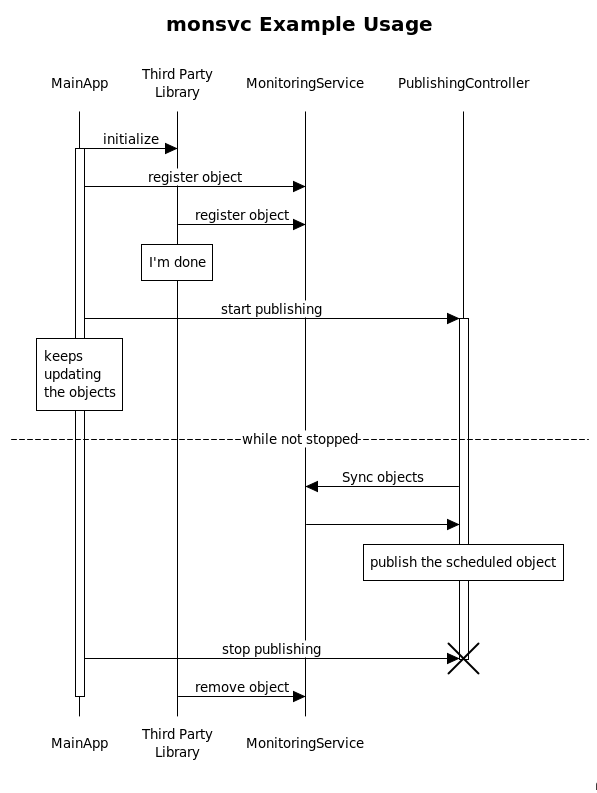
\includegraphics[scale=0.6]{Images/workflow.png}
\caption{{\tt monsvc} library usage example workflow.}
\end{figure}

The separation of registration and publishing also makes the life of third party library developers easier since their only job is to register the objects they want to be monitored while the main application is concerned with configuring and starting the publishing. For example, a network transport library will register information about the amount of trasferred data. This information will then be publsihed together with the main application data.

This usage pattern allows us to  create a lightweight version of the monsvc library with no transitive linking dependencies which contains only the registration functionality and which can be used by other libraries. The main application has to use the normal version which depends on a number of other packages like IPC, ROOT, IS, etc.
